% !TEX root = ../MasterThesis.tex

\chapter{深層学習の概観} \label{sec:DeepLearning}
本章では、深層学習技術について、その概観を述べる。
3.1節では基本的な深層学習の概観を述べる。%3.2節では深層学習と粒子物理学との関連について取り上げる。
3.2節でグラフニューラルネットワーク(Graph Neural Network, GNN)について紹介した後、3.3節で一般的なニューラルネットワーク(Neural Network, NN)の実装について説明する。

%この章では、PFAを改善させるために導入した深層学習技術について、その概観を説明する。3.1節では深層学習の対象として教師あり学習と教師なし学習の違いを説明する。3.2節では深層学習の最も基本的な構造であるパーセプトロンについて述べる。3.3節ではパーセプトロンを組み合わせることで構成される単純な深層学習ネットワークであるニューラルネットワークについて述べる。3.4節では、ニューラルネットワークを使用する際の学習の進行過程について述べる。3.5節ではニューラルネットワークを用いる際に、さらに精度を向上させるための種々の技術について述べる。3.6節ではニューラルネットワークをさらに応用したグラフニューラルネットワークについて説明する。

\section{深層学習}
%21世紀以降、情報処理技術や微細集積回路製造技術などの発達により取り扱うデータや解析により得られるデータは膨大かつ複雑になっている。

21世紀以降、取り扱うデータや解析により得られるデータは膨大かつ複雑になっていることが課題となっており、それまでの技術では処理に必要となるアルゴリズムが要求される性能に対して不十分となるケースが増えている。したがって新たな解析手法が必要となっており、その一つとして研究されてきたのが深層学習技術である。深層学習は機械学習の一種であり、この後に紹介するディープニューラルネットワーク(Deep Neural Network, DNN)だけでなく、敵対生成ネットワーク(Generative Adversarial Networks, GAN)やAuto-encoderなども深層学習技術に含まれる。深層学習技術の特徴としては、入力されてきたデータの特徴をより詳細に、より様々な観点から捉えるために、「深い」構造を持っていることが挙げられる。%機械学習の構想は人間の知能と同等の能力を保持する計算機として開発が期待されていた人工知能というアイデアに影響を受けているが、人間の頭脳のように複雑な構造を計算機上でアルゴリズムとして再現するために深層学習技術はより深く、より多くのデータ量を扱えるように進歩してきた。

深いネットワークを構築することで表現能力が上がり、より複雑な問題を扱うことができるようになる。これにより従来よりも速い処理速度で解析を行う精度の高いアルゴリズムを作成することが可能となった。
%この特徴の長所として、アルゴリズムに新たな構造を加えるのではなく、基本的な構造をより深くすることで従来の技術では到達できなかったデータ量の解析を行うことが期待される点である。これにより新たなアルゴリズムを考案することなく、アルゴリズムに含まれるパラメータの数を変更することで性能の向上が見込める。

深層学習の例として、図\ref{DNN}のように表され、入力層と出力層に多数の中間層を挿入したネットワークであるDNNを取り上げる。この技術は教師あり学習として利用され、回帰問題や分類問題に使用される。

\begin{figure}[h]
	\begin{center}
		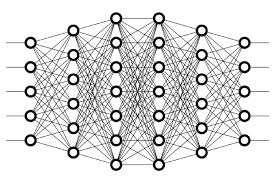
\includegraphics[width=250pt]{./Figure/DeepLearning/dl.jpeg}
		\caption[全結合DNNの模式図]{全結合DNNの模式図。}
		\label{DNN}
	\end{center}
\end{figure}


ここで、丸で表されている部分をノード、それらをつなぐ線をエッジと呼ぶ。エッジは各ノード間のパラメータを伝播し、ノードにおいてそのパラメータを元にした計算が行われているという過程が生じている。

入力として複数のベクトルからなるデータを考える。入力層と出力層の間では重み$\textbf{W}=\{\{w^0_1, w^0_2,\ldots, w_n^0\},\{w_1^1,w_2^1,\ldots ,w_n^1\},\ldots\}$とバイアス$\textbf{b}=\{b^0,b^1,\ldots\}$、そして非線形関数$h(x)$を通じた以下の計算が行われる。ただし、入力されたベクトルを$\textbf{x} = \{\{x^0_1, x^0_2,\ldots, x_n^0\},\{x_1^1,x_2^1,\ldots ,x_n^1\},\ldots\}$としている。
\begin{equation}
\textbf{y}  = h(\textbf{a}) = h(\textbf{Wx} +\textbf{b})
\end{equation}
ここで、重み$\textbf{W}$はサイズとして中間層の数と入力パラメータの数をもつ行列であり、その入力パラメータの寄与がどのくらい大きいかを表す一方、バイアス$\textbf{b}$は伝播してきたパラメータがどのくらい大きな寄与を示せば出力層へと伝播していくかの閾値を示しているとみなせる。また、ここで用いられている非線形関数を特に活性化関数と呼ぶ。

\begin{comment}
\begin{aligned}
\ h(\textbf{Wx} +\textbf{b})\\
\ h(\textbf{Wx} +\textbf{b})\\
\end{aligned}
\right.
\end{comment}

活性化関数についてはさまざまなものが提案されている。例えば、Rectified Linear Unit(ReLU)関数は
\begin{equation}
y = h(\textbf{a}) = \left\{
\begin{aligned}
0  \ (\textbf{a}  \le \theta)\\
\textbf{a}  \ (\textbf{a}  > \theta)\\
\end{aligned}
\right.
\end{equation}
と表され、入力が閾値を超えた後は入力に対して線形に増加する。他にも、双曲線関数$\tanh(\textbf{a})$やシグモイド関数$1/(1+\exp(-\textbf{a}))$などが用いられる。
これらの活性化関数を図\ref{act}に示す。

\begin{figure}[H]
	\begin{center}
		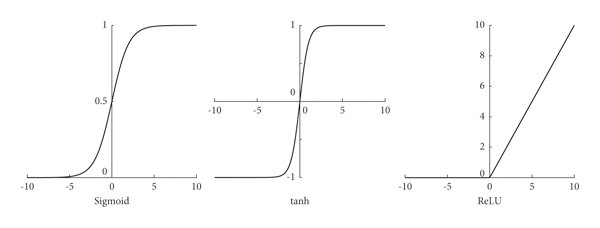
\includegraphics[width=350pt]{./Figure/DeepLearning/Output.jpeg}
		\caption[活性化関数の例。]{活性化関数の例。}
		\label{act}
	\end{center}
\end{figure}

深層学習の目的として、大きく分類問題と回帰問題の2種類が挙げられる。

分類問題は特徴量を持ったデータからそれぞれをいくつかの種類に識別する問題である。例として、手書き数字の画像を0から9までの数字に識別するMNIST問題が挙げられる。この課題では白黒、つまり0か1の数字で表現された手書き数字を離散的な出力$0~9$として分類する。

回帰問題はデータの特徴からその傾向について探り、連続的な変数を出力として得る問題である。

%どちらの種類の課題に対しても、深層学習は中間層を増やすことで表現能力が上がり、より多くの問題に対応できるようになるという特徴を持つ。

\section{Graph Neural Network}
Graph Neural Network (GNN)は深層学習技術の一つであり、グラフ構造を持ったデータの学習に有効であるという結果が得られている。グラフ構造を持ったデータは、DNNの説明でも述べたノードとエッジから構成されている。

グラフの構造として、いくつかの選択肢が存在する。
\begin{itemize}
\item エッジの向きの有無

2つのノードをつなぐエッジに対しては向きを設定することができる。向きを持ったグラフを有向グラフと呼び、持っていないものを無向グラフと呼ぶ。

通常、方向を持ったエッジはそうでないエッジに比べて情報量が多く、順方向と逆方向とで異なる特徴量を学習する。

\item グラフのノードの種類

全てのノードおよびエッジの種類が同じものを同種グラフ、複数の種類が混在しているものを異種グラフと呼ぶ。

\item 時間の経過に伴うグラフの変化

学習によってグラフの構造が変化する場合を動的グラフ、そうでない場合は静的グラフと呼ばれる。

\end{itemize}

また、学習を行う対象として幾つかの種類が存在する。
\begin{itemize}
\item ノードレベル 

各ノードを分類したり、ノード回帰の計算を行う。

\item エッジレベル

エッジごとの種類を分類するエッジ分類やエッジが存在するかしないかを予測するリンク予測などが挙げられる。

\item グラフレベル

グラフ全体の分類や回帰問題に関する問題を取り扱う。
\end{itemize}


GNNはノードとエッジの関連性に着目し、その特徴と関係性を学習することでグラフデータの解析を行うことが可能となる。応用例として、グラフベースで扱うことのできる化合物・生物分子解析、論文ごとの関連性、交通・物流予測などにおいて活用が図られている。

素粒子実験の分野ではグラフベースで扱えるものが少なくなく、現在GNNによる物理解析の研究が盛んになりつつある。例として、飛跡検出器で捉えられたヒットをノードに、飛跡をエッジとして考えることで検出器応答をグラフとして表せる。与えられたデータの特徴量をグラフとして与えるためには、グラフ構造の設計を考え適切なものを選択する必要がある。その際、ノードとエッジとして表現される対象に応じてGNNアーキテクチャの構造を選択することで最適な精度を得ることができる。


\section{ニューラルネットワークの実装}
GNNに限らず、ニューラルネットワークの実装には以下のいくつかの手順が必要となる。

\begin{enumerate}
\item データ準備

入力データは解析の精度を高める上でも重要であり、GNNの場合はグラフの形状に合わせたデータセットを用意する必要がある。深層学習においては前処理としてデータを$[-1,1]$の範囲に制限することでより精度の高い解析が可能となるケースが多い。

データは訓練データ、評価データに分割し、それぞれ別々の用途に用いる。

\item モデル作成

目的とするタスクおよびデータの特徴に応じた適切なネットワークモデルを選択する。

GNNの一つとして、計算の高速化と汎用化のために開発されたのがMessage Passingと呼ばれるネットワークである。
以下、入力パラメーターによってノード特徴量$x_v$、エッジ特徴量$e_{vw}$をもつ無向グラフGが構成されたとする。学習ステップを$\{t|t\in T\}$で表す。それぞれのノードには隠れ状態$h_v^t$が設定されており、Message Passingでは
\begin{equation}
m_v^{t+1} = \sum_{w \in N(v)} M_t(h^t_v,h^t_w,e_{vw})
\end{equation}
\begin{equation}
h_v^{t+1} = U_t(h_v^t,m_v^{t+1})
\end{equation}
のようにグラフの特徴量を伝達し、パラメータを更新する。

ここで、$N(v)$はインデックスvを含むノードおよびエッジに接続されている要素を示し、$M_t$および$U_t$はネットワークに固有の関数であり、それぞれメッセージ関数とノード更新関数と呼ばれる。

最終的な出力は読み出し関数$R$を用いて
\begin{equation}
\hat{y} = R(\{h_v^T | v \in G\})
\end{equation}
と得られる。

関数$M_t$、$U_t$、$R$は全てネットワークの学習によって得られる関数であり、隠れ状態$h_t$を通じて入力パラメータから得られる。
Message PassingはGraph Convolutional Networks(GCN)やNeural Fingerprint(NF)といったその他のGNNの構造をこれらの関数によって一般化したものと考えられる。

例えば、Convolutional Networkの1つはMessage Passingにおいて
\begin{equation}
M(h_v,h_w,e_{vw}) = \mathrm{concatenate}(h_w,e_{vw})
\end{equation}
\begin{equation}
U_t(h_v^t,m_v^{t+1}) = \sigma(H_t^{\mathrm{deg}(v)}m_v^{t+1})
\end{equation}
(ただし、$\sigma$はシグモイド関数、$\mathrm{deg}(v)$はノード$v$の数、$H_t^N$はステップ$t$、ノード数$N$の時の学習によって得られた行列を指す。)
\begin{equation}
R = f(\sum_{v,t} \mathrm{softmax(W_th_v^t)})
\end{equation}
(ただし、$f$はニューラルネットワーク、$W_t$は学習によって得られた読み出し行列を指す。)

のように関数を定義した場合と同様である。

ネットワークとしてBatch Normalizationと呼ばれる手法を用いることがある。この手法はレイヤーごとに特徴量を規格化することで過学習を避けるための方法となっている。まず、出力されてきたバッチから平均と分散を計算する。出力を$x_i$、出力の数を$m$とすると、平均$\mu_B$および分散$\sigma_B^2$は
\[
\mu_B = \frac{1}{m}\sum_{i=1}^m x_i
\]

\[
\sigma_B^2 = \frac{1}{m}\sum_{i=1}^m(x_i-\mu_B)^2
\]

となり、この値を用いて出力として
\begin{equation}
\hat{x_i} = \frac{x_i - \mu_B}{\sqrt{\sigma_B^2+\epsilon}}
\end{equation}
のように規格化される。
ここで分母に微少量$\epsilon$を加えることにより$\sigma_B^2$が小さくなってしまいゼロ除算が発生することを防いでいる。
こうして求められたバッチデータに対して線形変換
\begin{equation}
y_i\leftarrow\gamma\hat{x_i}+\beta
\end{equation}
を行うことで、平均$\beta$、標準偏差$\gamma$の正規分布が得られる。

\item モデル学習

学習に必要となる損失関数とその最適化手法を決定し、実行する。
損失関数とはネットワークから出力されてきた数値と正解ラベルとのズレを示す関数であり、NNからの出力を$y_k$、正解ラベルを$t_k$とすると回帰問題に使用される二乗和誤差関数(Mean Squared Error)
\[
L=\frac{1}{2}\sum_k (y_k-t_k)^2
\]
と分類問題において使用される交差エントロピー誤差(Cross Entropy Error)
\[
L=-\sum_k t_k\log(y_k)
\]
が主に挙げられる。

損失関数$L(\textbf{W})$の重みパラメータ$\textbf{W}$による勾配を得るために取られる有用な手法が誤差逆伝播法である。

\begin{comment}
順方向のニューラルネットワークの計算は
\[
\textbf{y} = h(\textbf{Wx} + \textbf{b}) 
\]
であったが、
\end{comment}
%勾配を計算するためには$\textbf{W}$と$\textbf{x}$が必要である。
順方向の損失関数までの伝播を模式的に表したものを図\ref{BackProp}に示す。
なお、この図は計算グラフと呼ばれるニューラルネットワークの計算の過程を視覚的なグラフで表したものである。

\begin{figure}[H]
	\begin{center}
		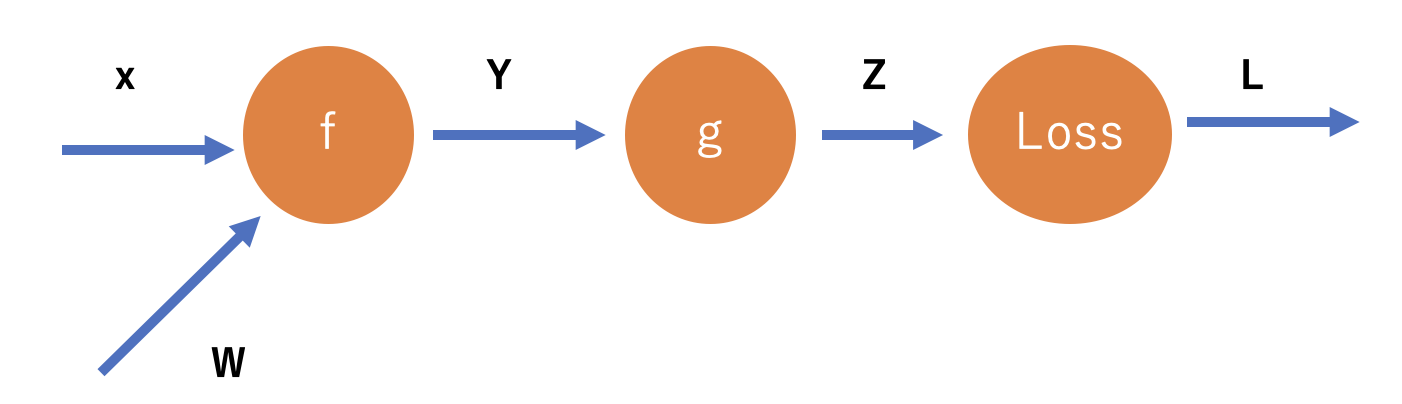
\includegraphics[width=350pt]{./Figure/DeepLearning/BackProp.png}
		\caption[順方向の伝播を示す計算グラフ]{順方向の伝播を示す計算グラフ。}
		\label{BackProp}
	\end{center}
\end{figure}

計算グラフはこれら一連の計算によって損失関数$L$が
\begin{equation}
L = \textrm{Loss}(g( f(\textbf{x}, \textbf{W}))) = \textrm{Loss}(g(\textbf{Y})) = \textrm{Loss}(\textbf{Z})
\end{equation}
と順々に計算されている様子を表している。

%ニューラルネットワークでは$f(x)$は関数$f(\textbf{W}, \textbf{x}) =\textbf{W}\textbf{x}$、$g(x)$は関数$g(\textbf{W}\textbf{x}, \textbf{b})=\textbf{W}\textbf{x}+\textbf{b}$、そしてLossはシグモイド関数などの非線形関数に対応する。

%非線形関数$h(x)$からの出力をそれぞれ$\textbf{Y}$、$\textbf{Z}$とし、ロスを$L$とすると
今回、損失関数$L$の重み$\textbf{W}$に対する勾配を考えたいので、各出力による微分を考える。この際、誤差逆伝播法によると$\textbf{x}$、$\textbf{W}$、$\textbf{Y}$、$\textbf{Z}$に対する逆伝播はそれぞれ図\ref{BackProp_back}のように表される。

\begin{figure}[H]
	\begin{center}
		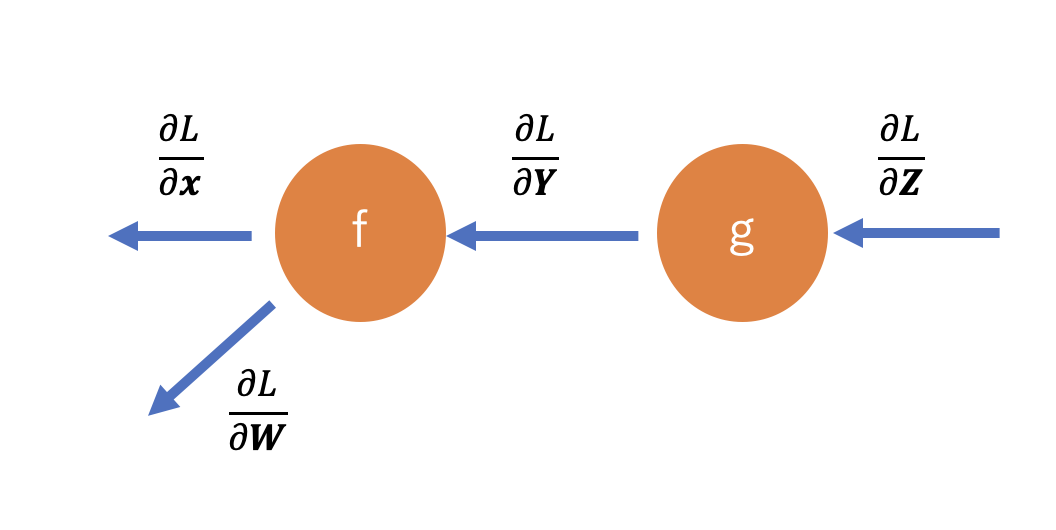
\includegraphics[width=350pt]{./Figure/DeepLearning/BackProp_back.png}
		\caption[逆伝播の模式図]{逆伝播の模式図}
		\label{BackProp_back}
	\end{center}
\end{figure}

1つのノードから2本の有向エッジが伸びている場合に、一方を計算するためにはもう片方のエッジとノードに入力されてきたエッジとの積を計算する。
すなわち、勾配$\frac{\partial L}{\partial \textbf{W}}$を得るためには
\begin{equation}
\frac{\partial L}{\partial \textbf{W}} = \frac{\partial L}{\partial \textbf{x}} f\left(\frac{\partial L}{\partial \textbf{Y}}\right)
\end{equation}
を計算する。
よって、求めたい勾配は損失関数から
\begin{equation}
\frac{\partial L}{\partial \textbf{W}}= \frac{\partial L}{\partial \textbf{x}}\cdot f\left(g\left(\frac{\partial L}{\partial \textbf{Z}}\right)\right)\end{equation}
と得られる。
なお、合成関数の微分から、右辺は
\begin{equation}
\frac{\partial L}{\partial \textbf{W}} = \frac{\partial }{\partial \textbf{x}}\left(f\left(g\left(\frac{\partial L}{\partial \textbf{Z}}\right)\right)\right)
\end{equation}
とも表される。

勾配を得るための方法として、重みパラメータそれぞれに関して損失関数の数値微分を行うことも可能だが、計算が非常に膨大になるため、実用的には誤差逆伝播法が用いられる。

最適化手法の一つとして、RMSPropを説明する。
誤差逆伝播法の結果から、
%重み$\textbf{w}^{(t)}$に依存した損失関数$L(\textbf{w}^{(t)})$が得られたので、
この損失関数の勾配$\textbf{g}^{(t)}$に沿って損失関数を低減させることでネットワークから出力されてきた値を正解ラベルへと近づけることができる。

勾配$\textbf{g}^{(t)}$は
\[
\textbf{g}^{(t)} = \Delta L(\textbf{W}^{(t)})
\]
である。RMSPropでは、パラメータ$\textbf{v}_{(t)}$を導入し、重みパラメータを更新する前に
\[
\textbf{v}_{(t)}=\rho\textbf{v}_{(t-1)}+(1-\rho)(\textbf{g}^{(t)})^2
\]
を計算する。
この$\textbf{v}_{(t)}$を用いて重みパラメータの勾配$\Delta\textbf{W}^{(t)}$を
\[
\Delta\textbf{W}^{(t)}=-\frac{\eta}{\sqrt{\textbf{v}_t+\epsilon}}\textbf{g}^{(t)}
\]
と計算し、新たな重みパラメータ
\[
\textbf{W}^{(t+1)} = \textbf{W}^{(t)}+\Delta\textbf{W}^{(t)}
\]
が得られる。RMSPropは先に行われていた重みパラメータの更新が後のパラメータ更新へ影響を与えにくくなるため、学習の間で勾配変化の大きい場合の学習に適している手法である。これを応用してAdamやAdamWといったさまざまな最適化手法が考案されている。


\begin{comment}
合成関数の微分と最適化アルゴリズムを用いて得られた$\Delta\textbf{W}^{(t)}$を用いて
\frac{\partial L}{\partial y_{ij}} = \sum_{k,l}\frac{\partial L}{\partial z_{kl}} \frac{\partial z_{kl}}{\partial y_{ij}}
\end{comment}


\begin{comment}
\[
 \frac{\partial E}{\partial w_{jk}} = h'_k(w_k x_k)\frac{\partial E}{\partial y_k}y_j
\]
を得る。ただし、$w_{jk}$は重みパラメータ$\textbf{W}$のjk成分。$x_j$および$x_k$$y_j$および$y_k$はそれぞれ出力$\textbf{x}$、$\textbf{y}$のj,k成分。
\end{comment}



%選択されたモデルによって出力が得られた後、損失関数の計算が行われ、最適化手法によりパラメータが調整される。全てのデータを用いてパラメータが調整されるタイミングが1エポックと呼ばれ、学習回数を表す単位の一つとなる。



\item モデル評価

訓練データ、評価データを用いてネットワークの評価を行う。
\begin{itemize}
\item 推論性能評価

全ての評価データのうち、正しくネットワークが判別できているデータの割合を推論精度(Accuracy)と呼び、ネットワークによる推論の確らしさを示している。
\item  汎用性能評価

訓練データと評価データに対する損失関数の学習進度ごとの変化から、汎化推論精度を確認することができる。訓練データのみの損失関数が減少している場合、ネットワークの汎化性能は低いと言える。なお、学習進度を示す単位として、訓練データを何回繰り返したかをエポック(epoch)と呼ぶ。

\end{itemize}

\end{enumerate}










%%%%%%%%%%%%%%%%%%%%%%%%%%%%%%%%%%%%%%%%%%%%
\begin{comment}
\subsection{教師あり学習と教師なし学習}
機械学習は与えられた特定のデータから目的とする正解データをアルゴリズムにより導くための技術である。深層学習は深層ニューラルネットワークを利用した機械学習技術の一部に位置づけられる。機械学習の対象となる課題には、教師あり学習と教師なし学習に分けられる。教師あり学習では、まず入力となるパラメータと正解ラベルを持つデータが与えられ、その相関関係を元にして目的となるデータの予測ラベルを出力する。一方、教師なし学習では正解ラベルを与えられることなしに入力パラメータのみから予測ラベルの推定を行う。今回目的とするカロリメータークラスタリングのような解析は前者が有効となる。他方でロボットの制御やビデオゲームにおける最適行動解の探索などには強化学習として、後者が用いられることがある。


\subsection{単純パーセプトロン}

単純パーセプトロンは図のような入力層と出力層のみを持つ単純なネットワークである。このネットワークに入力パラメータを$x_1$、$x_2$が与えられると、重み$w_1$、$w_2$を乗算して和をとった$w_1x_1+w_2x_2$が計算され、出力層には非線形関数$h(x)$を通じて出力$y$が求められる。$h(x)$は単純パーセプトロンの場合はヘヴィサイドの階段関数と呼ばれる閾値$\theta$を持った関数が用いられ、
\begin{equation}
y = h(a) = \left\{
\begin{aligned}
0  \ (a = w_1x_1 + w_2x_2 \le \theta)\\
1  \ (a = w_1x_1 + w_2x_2 > \theta)\\
\end{aligned}
\right.
\end{equation}
ここで、重み$w_1$、$w_2$はその入力パラメータの寄与がどのくらい大きいかを表し、バイアス$\theta$はそのパラメータがどのくらい大きな寄与を示せば出力層へと伝播していくかの閾値を示しているとみなせる。また、出力層に伝播する際に使用される非線形関数を特に活性化関数と呼ぶ。一層だけの単純パーセプトロンでは極めて限られたケースしか取り扱えないがこれらを組み合わせることで、次の節で紹介するニューラルネットワークとして応用範囲を広げることができる。


\subsection{ニューラルネットワーク}
中間層を増やすことで表現能力が上がり、より多くの問題に対応できるようになっている。重みの計算は単純パーセプトロンの場合と同様だが、出力層において用いられる非線形関数についてさまざまなものが提案されている。例えば、Rectified Linear Unit(ReLU)関数は
\begin{equation}
y = h(a) = \left\{
\begin{aligned}
0  \ (a  \le \theta)\\
a  \ (a  > \theta)\\
\end{aligned}
\right.
\end{equation}
と表され、入力が閾値を超えた後は入力に対して線形に増加する。他にも、双曲線関数$\tanh(a)$やシグモイド関数$1/(1+exp(-a))$などが用いられる。
中間層が多く存在するニューラルネットワークを深層ニューラルネットワークと呼び、このような深いネットワークを用いて学習することを特に深層学習としている。


\subsection{損失関数}

\subsection{誤差逆伝播}


深層教師あり学習には大きく分けて5つの段階が存在する。
\begin{itemize}
\item データをネットワークに適切な形式となるように整形する
\item 入力データをネットワークに入れてその出力と正解ラベルとの差を比較する
\item その差を元にして誤差逆伝播法によりネットワークの重みやバイアスを学習する
\item 上記2 - 3を誤差が最適となるまで繰り返す
\item 評価データを用いてネットワークの性能を評価する
\end{itemize}

これらの過程を通じて入力データから出力データの値を推定する。


\section{精度向上のための技術}
ニューラルネットワークの問題点の一部が勾配消失や過学習である。前者は損失関数を計算するときにその勾配計算ができなくなり、学習が進まなくなる現象である。一方、後者はネットワークが訓練データに適合しすぎて、評価データに対して適切に出力できなくなる問題である。特に深いネットワークでは、これらの問題が起こりやすい。解決策としては、バッチノーマリゼーションや重み初期値の変更、ハイパーパラメータチューニングが挙げられる。バッチノーマリゼーションは各レイヤーの間にバッチ層を挟み、入力されてきたパラメータを規格化するという手法である。また、学習を行う前のネットワークの重み初期値をXavierの初期値などを使うことで改善することもできる。さらに、ネットワークに含まれるレイヤーの数や学習率などのパラメータはハイパーパラメータと呼ばれ、学習の際には一意に決められている。このパラメータをさまざまに帰ることでネットワークの性能が変化しうる。この調整をハイパーパラメータチューニングと呼ぶ。


\section{グラフニューラルネットワーク}
グラフニューラルネットワーク(GNN)はニューラルネットワークにグラフの概念を利用することで、それぞれのデータの関係性がグラフによって表される場合に、その関係性を学習に活用することを可能にするネットワークである。グラフは各特徴量を保持するノードと、それぞれの特徴量の関係を表すエッジによって構成され、ノードの種類が同じグラフをホモジーニアス、異なるグラフをヘテロジーニアスと呼ぶ。応用例としてはグラフベースで扱うことのできる、化合物・生物分子解析、論文ごとの関連性、交通・物流予測などが挙げられる。
\end{comment}
%%%%%%%%%%%%%%%%%%%%%%%%%%%%%%%%%%%%%%%%%%%%%
